\section{Correction using timing beacon on satellite}

\begin{figure}[ht!]
	\begin{minipage}{.4\textwidth}
		The timing beacon correction method installs a beacon with regular pulses on the satellite. We time-stamp the beacon signal both on the satellite and at the ground station (Fig \ref{fig:beacon}). By introducing structure, we can warp the time-stamps until the beacon pulses match up, and then apply the same transformation to the idler and signal photoevents.
		
	\end{minipage}
	\begin{minipage}{.6\textwidth}
		\centering
		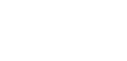
\includegraphics[width=0.9\linewidth]{assets/beacon}
		\caption{The beacon setup.}
		\label{fig:beacon}
	\end{minipage}%

\end{figure}


The higher order correction calculates the clock drift for each point and uses a second order polynomial fit to determine the clock drift at each point. For the case of 90 degrees elevation, this is shown below:

\begin{figure}[ht!]
	\centering
	\includegraphics[width=0.7\linewidth]{assets/beacon_alex}
	\caption{Estimation of the second-order correction at each point.}
	\label{fig:beacon_alex}
\end{figure}

We find that even a high jitter beacon with poor detection efficiency is sufficient to correct for all clock drifts including the change of the Doppler shift for high elevation angles.

However, the beacon introduces additional requirement into the satellite's payload. By using information from the TLE and methods like gradient ascent, we can recover the shift without the additional structure of beacon pulses.

